%\documentclass[preprint,authoryear,11pt]{elsarticle}
\documentclass[preprint,authoryear,11pt,5p,times,twocolumns]{elsarticle}
\usepackage{amssymb}
\usepackage{amsmath}
\usepackage{graphicx}
\journal{Journal of Neuroscience}
\usepackage{hyperref}
\usepackage{lineno}
\hypersetup{ colorlinks=true, urlcolor=blue}
 \hyphenation{wide-spread tar-get}

\begin{document}

\begin{frontmatter}

\title{Proactive and reactive control processes involve dynamic reorganisation of alpha and theta oscillatory networks}
\author[label1,label2,label3]{Patrick S. Cooper}
\author[label2,label4]{Aaron S.W. Wong}
\author[label1,label2,label3]{Elise Mansfield}
\author[label1,label2,label3]{W. Ross Fulham}
\author[label1,label2,label3]{Patricia T. Michie}
\author[label1,label2,label3]{Frini Karayanidis}
\address[label1]{School of Psychology, Universtiy of Newcastle}
\address[label2]{Functional Neuroimaging Laboratory, University of Newcastle}
\address[label3]{Hunter Medical Research Institute, University of Newcastle}
\address[label4]{School of Engineering, University of Newcastle}

\begin{abstract}
Lorem ipsum dolor sit amet, consectetur adipiscing elit. Donec a diam lectus. Sed sit amet ipsum mauris. Maecenas congue ligula ac quam viverra nec consectetur ante hendrerit. Donec et mollis dolor. Praesent et diam eget libero egestas mattis sit amet vitae augue. Nam tincidunt congue enim, ut porta lorem lacinia consectetur. Donec ut libero sed arcu vehicula ultricies a non tortor. Lorem ipsum dolor sit amet, consectetur adipiscing elit. Aenean ut gravida lorem. Ut turpis felis, pulvinar a semper sed, adipiscing id dolor. Pellentesque auctor nisi id magna consequat sagittis. Curabitur dapibus enim sit amet elit pharetra tincidunt feugiat nisl imperdiet. Ut convallis libero in urna ultrices accumsan. Donec sed odio eros. Donec viverra mi quis quam pulvinar at malesuada arcu rhoncus. Cum sociis natoque penatibus et magnis dis parturient montes, nascetur ridiculus mus. In rutrum accumsan ultricies. Mauris vitae nisi at sem facilisis semper ac in est. Vivamus fermentum semper porta. Nunc diam velit, adipiscing ut tristique vitae, sagittis vel odio. Maecenas convallis ullamcorper ultricies. Curabitur ornare, ligula semper consectetur sagittis, nisi diam iaculis velit, id fringilla sem nunc vel mi. Nam dictum, odio nec pretium volutpat, arcu ante placerat erat, non tristique elit urna et turpis. Quisque mi metus, ornare sit amet fermentum et, tincidunt et orci.
\end{abstract}

\begin{keyword}
cognitive control, \ coherence, \ oscillatory synchronisation, \ functional connectivity, \ task switching, 
\ theta, \ alpha
\end{keyword}

\end{frontmatter}
\section{Introduction}

Cognitive control processes allow us to adjust our behaviour flexibly in order to meet internal motivations or goals. Depending on contextual constraints, this control can be adopted either proactively, pre-setting the system to be sensitive to goal-relevant features of the environment or reactively, responding to such goal-relevant features on a needs basis \citep{Braver}.  The implementation of these control processes is known to rely on an extensive and well-described frontoparietal communication architecture \citep{Corbetta,Seeley,Vincent} that is well-suited to promote flexible and rapid information propagation \citep{Dosenbach}. Yet, despite the increasing knowledge regarding the anatomical architecture that permits flexible control, the functional properties of this network are less well characterised. 


One plausible mechanism by which information can be flexibly adjusted and rerouted in the frontoparietal network is oscillatory synchronisation. Separate populations of neurons are able to exchange information transiently by synchronising the excitability windows in which they are most sensitive to electrical influxes \citep{Fries,Womelsdorf}.  Such synchronisation produces assemblies of neurons that are functionally connected for a given period of time. The neurons in these assemblies oscillate rhythmically, allowing receiving and transmitting components to precisely time their firing rates, and thereby achieving an efficient mechanism to exchange information within the assembly that is also less sensitive to competing inputs from alternative assemblies \citep{Azouz,Engel}.  Indeed, oscillatory synchronisation has been shown to be functionally relevant in numerous higher-order cognitive processes such as working memory \citep{Huang,Palva2005,Pesonen,Sauseng2005,Wu}, 
\nopagebreak selective attention \citep{Doesburg2,Doesburg,Kahlbrock,Maris} and inhibition \citep{Papenberg,Serrien,Tallet}. By transiently synchronising activity within the frontoparietal network, goal-relevant representations may be afforded an elevated processing status that permits effective cognitive control.  


The evidence for the role of oscillatory synchronisation in cognitive control is currently largely restricted to slow wave, theta (4-7Hz) synchronisation in goal and response conflict resolution. For example, increases in theta synchronisation have been reported in paradigms requiring error detection and post-error correction \citep{Cavanagh,Luu,Trujillo}, goal conflict and response selection \citep{Moore2006, Moore2012}, as well as in task switching \citep{SausengTSWT}. As these goal-relevant processes are important contributors to cognitive control \citep{Miyake}, these findings suggest that theta oscillations may be a neural signature of goal-directed processes. 


Interestingly, the role of theta in cognitive control has been investigated almost exclusively using paradigms that do not differentiate between proactive and reactive control. For example, Sauseng and colleagues reported widespread frontoparietal coherence in the theta band when participants switched randomly between digit magnitude and digit classification tasks compared to repeating one of these tasks \citep{SausengTSWT}. Here, there was no advance information about whether the upcoming trial would require a switch or a repeat in task. Instead, the stimulus had to first be encoded to decide which task needed to be implemented (e.g., repeat the same task or change to alternative task) and secondly to implement that task in the presence of competing information (e.g., respond smaller/greater than 5, ignore parity). Likewise, when participants were searching for a specific rule (i.e. the presentation of four odd digits) frontoparietal theta connectivity was observed during each instance that this rule was not met (i.e. goal conflict) as well as correct detection - response selection \citep{Moore2006}. Other studies investigating the role of theta synchronisation in cognitive control have also used paradigms that do not differentiate between proactive and reactive control (e.g., Flanker tasks in \citealt{Cavanagh}). 


In fact, studies that have specifically targeted proactive control, by examining electrophysiological activity in the cue-target interval, i.e., the interval between an informative cue to switch or repeat task and the subsequent target, have shown changes not in theta, but in alpha (8-13Hz) power \citep{Mansfield2012} and oscillatory synchronisation \citep{Serrien}. Together, these findings suggest that proactive and reactive cognitive control modes may involve distinct neural processes. As functionally relevant neural coupling often occurs between frequencies \citep{Jensen}, perhaps the frontoparietal control architecture dynamically shifts between theta and alpha oscillatory synchronisation depending on contextual demands.

The current study aimed to investigate the potential mechanistic dissociation between proactive and reactive control via alpha and theta oscillatory synchronisation respectively. To do so, we utilised a cued-trials task switching paradigm where we manipulated the ability to prepare for a repeat or switch between simple classification tasks (\citealt{Karayanidis2009}; see Methods). This manipulation allowed us to disentangle proactive, reactive and switch-related processes to explore the role of alpha and theta oscillatory synchronisation in cognitive control. Based on this separation of control processes, if theta synchronisation is associated with switching (cf. \citealt{SausengTSWT}) then we expect to see increases in frontoparietal coherence during switch aniticpatory processes and/or target-based switch processes specifically. However, if theta synchronisation is an index of reactive control, extensive frontoparietal connectivity should occur only after target onset in those conditions advance preparation was insufficient for. Given previous findings suggestive of a role of alpha oscillatiory activity in switch preparation, we also expect to see the frontoparietal network utilise alpha frequencies when preparing for any switch in task rather than a task repeat.

\section{Methods}

\subsection{Participants}

Twenty-nine (13 male, mean age 25.69 $\pm$5.64 years) young adults from the Newcastle community took part in the current study as part of a larger project (\href{http://www.age-ility.org.au/}{http://www.age-ility.org.au}) and received \$20 per hour reimbursement. All participants were asked to abstain from caffeine and alcohol prior to testing, were right-handed and had no current neurological or psychiatric disorder. The University of Newcastle Humans Ethics Research Committee approved the current study. 

\subsection{Stimuli and Task}

To characterise proactive and reactive control networks, we utilised a cued-task switching paradigm containing task-repetition and task-set changes with varying degrees of preparation. A grey wheel ($5\,^{\circ}$ diameter) was presented continuously with six equal-sized segments. Two adjacent segments were considered a major sub-division of the wheel and were associated with one of three classification tasks: a letter classification task (\textit{vowel/consonant}), a digit classification task (\textit{odd/even}) and a colour classification task (\textit{hot/cold}; see Figure 1). Participants were presented a bivalent target in one of the two segments associated with the task and were instructed to classify the task-relevant features using a left or right button press. Targets contained one task-relevant dimension (e.g. for the letter task, the vowel 'A'), one incongruently response-mapped feature (e.g. an even digit '4') and a third neutral feature (e.g. a grey target 'A4'). The same target could not appear on successive trials, the same trial type could not be repeated more than four consecutive times and response mappings were counterbalanced between participants (Figure 1).


To assist in preparing for the upcoming target, two adjacent segments of the wheel were bolded for 1000ms prior to target onset, with the target appearing in one of the two cued sections. If the cue highlighted two segments that exclusively belonged to only one of the three classification tasks, these cues were considered to be \textit{informative}. An informative cue could indicate a repetition of a task, a \textit{repeat} trial or a change in task, a \textit{switch-to} trial. If the two cued segments overlapped with more than one classification task (e.g. a section belonging to the digit and a section belonging to the colour task were highlighted) then complete preparation for the upcoming target was unable to occur. If the two sections cued were from tasks that were not completed on the previous trial, this indicated a change in task-set but not the identity of the task - a \textit{switch-away} trial. On these trials, switch but not task-set reconfiguration processes could occur. Alternatively, if the sections cued were from both the previous trial's task and another classification task, no maintenance, switch or task-set anticipation could occur and so these trials were deemed \textit{noninformative}. Taken together, proactive control was able to be employed for \textit{repeat} and \textit{switch-to} trials; \textit{switch-away} and \textit{noninformative} classification relied on reactive control and \textit{switch-to} and \textit{switch-away} trials reflected varying degrees of informative switching processes.

\begin{figure}[ht!]
\centering
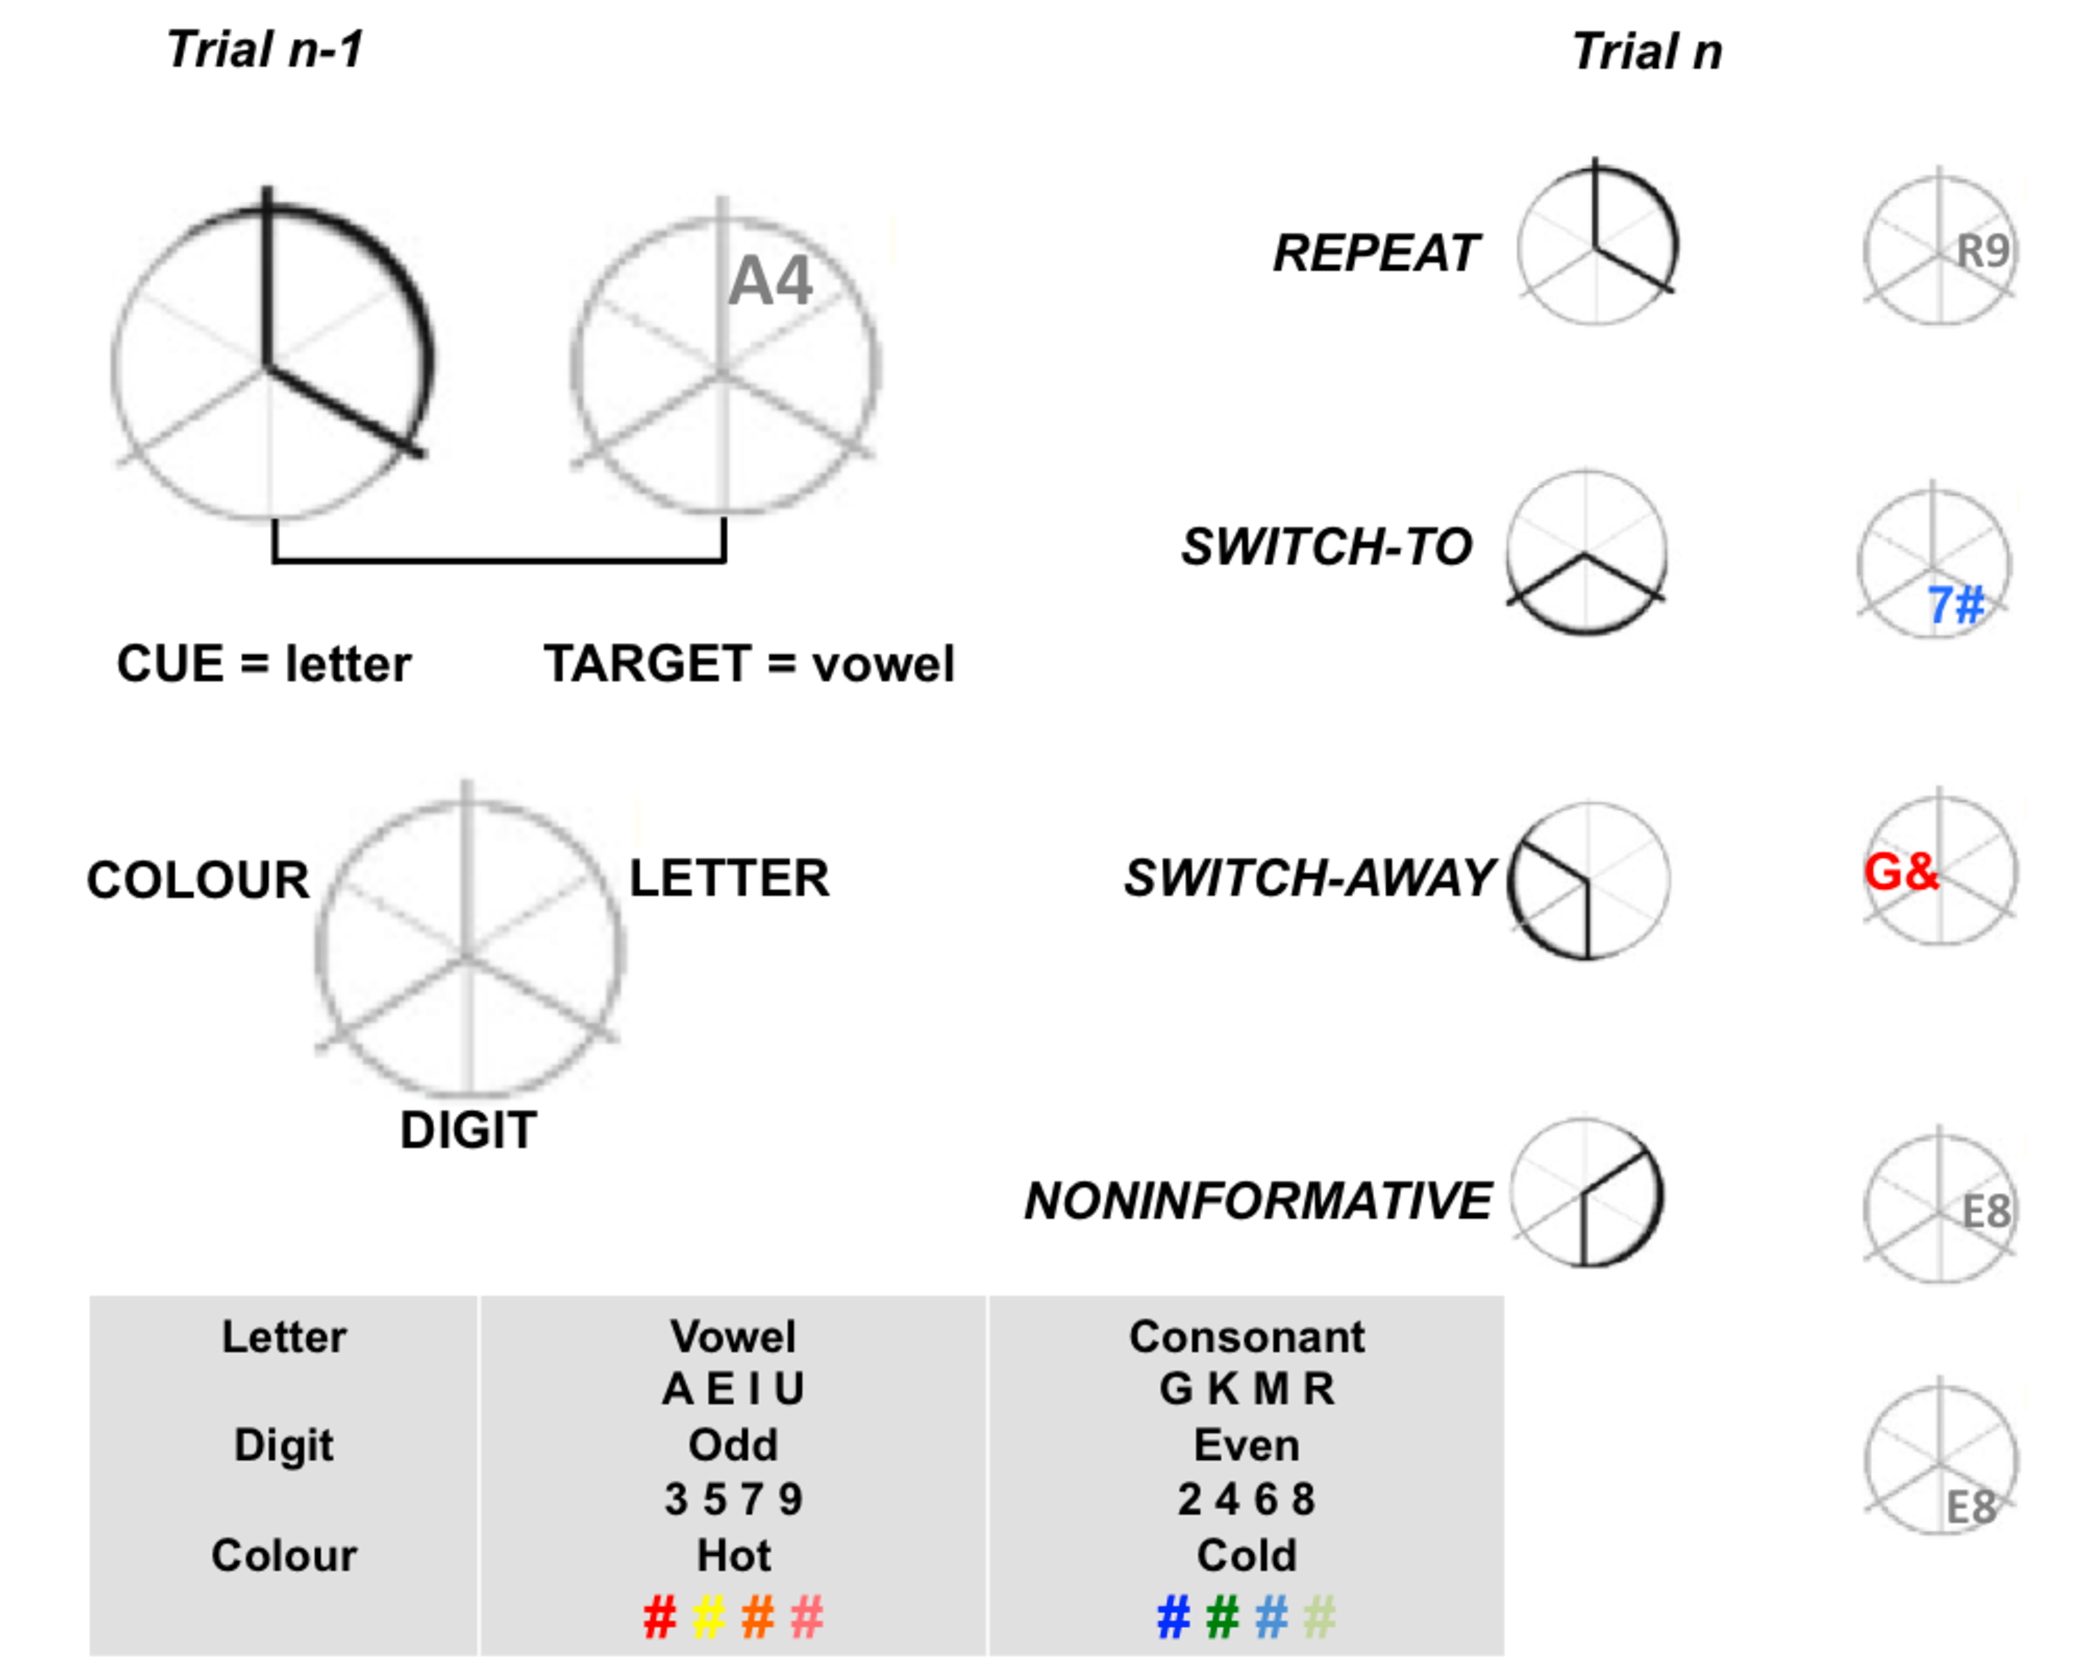
\includegraphics[width=90mm]{Figure1.pdf}
\caption{Cued-trials task switching paradigm. The current (\emph{Trial n}) condition (\emph{Repeat, Switch-to, Switch-away, Noninformative}) is dependent on the previous trial (\emph{Trial n-1}). Each major section of the wheel is associated with a classification task - letter/digit/colour. Left and right hand responses are mapped to one classification dimension for each task (an example response-mapping is shown here).}
\label{Paradigm}
\end{figure}

\subsection{Procedure and EEG Recording}

Prior to the experimental session participants learnt and practiced both single-task and switching blocks over two training sessions, one on initial contact and one prior to the EEG recording comprising 1320 practice trials total. Initial task learning occured no more than 14 days before the experimental session. For the experimental session, participants performed ten mixed task blocks and three single task blocks, in a dimmed testing room with simultaneous EEG recorded. Mixed task blocks comprised 72 trials (plus five dummy trials) and single task blocks 48 trials (plus five dummy trials). Only mixed task block data are presented here. For each trial a cue was presented for 1000ms which
disappeared at target onset where the target remained until response (or a five second time-out). A 600ms interval was inserted between response and the next cue. Error feedback was provided to participants via a tone. Reaction times and accuracy for each block were presented during inter-block feedback alongside a brief entertaining video. These breaks were semi-self paced, with participants informing the experimenter when they were ready to proceed to the next block. This was done to minimise fatigue effects.

EEG was recorded continuously at a sampling rate of 2,048Hz from 64 scalp electrodes and eight external leads (two outer canthi of the eyes, two supraorbital, two infraorbital, and left and right mastoids) using an ActiveTwo Biosemi EEG system. Data was recorded with reference to the common mode signal (CMS) and right driven leg (DRL) electrodes. 

\subsection{Data Analysis}

Behavioural and EEG data were processed offline. Responses faster than 200ms or slower than three standard deviations from each individual's mean RT were excluded from analyses. Post-error trials and those with unsuitable noise levels (see below) were additionally excluded from EEG analyses.

\subsection{EEG Analysis}

EEG data were processed using MATLAB 2011b (The Mathworks, Inc.) through a custom-built pipeline utilising Fieldtrip \citep{Oostenveld}, EEGLab \citep{Delorme} and in-house functions (see Figure 2). EEG data were initially read into Fieldtrip, using a common average reference and filtered (high pass: 0.1Hz, forward phase, 50Hz notch, zero phase). Data were visualised for noisy channels and if any were detected, interpolated using a \textit{k} nearest-neighbour approach. Trials (repeat, switch-to, switch-away, noninformative) were defined with respect to cue onset (from -1,000ms to +3,500ms). Independent components analysis (ICA) was performed to remove EOG-related artefact using the \textit{fastica} function (Hyv\"{a}rinen \& Oja, 2000). Before ICA was ran, trials were inspected and removed if their variance suggested they were an outlier, they had a value of over 1,000~$\mu$V or a \textit{z-value} \textgreater 4, in an attempt to make the strongest ICA-derived componets EOG-related. After EOG signals were removed from the data, trials underwent a second phase of artefact rejection where they were filtered with a low pass filter of 30Hz to remove remaining EKG artefacts, trials larger than $\pm$100$\mu$V automatically removed and a final inspection of trial variance to remove any remaining outliers. This approach typically resulted in 6\% ($\pm$9.1 SD) of trials removed. Finally, as coherence analyses were undertaken at sensor space, trials were transformed using scalp surface Laplacian estimates or current source density (CSD). CSD minimises volume conduction effects at EEG sensor space by removing large common signals across sites (spatial autocorrelation). Additionally, CSD is a reference-free montage which eliminates artificial coherence between electrodes due to a shared reference, providing a more sensitive connectivity measure that is relatively uninfluened by common sources and reference montage problems.
\begin{figure}[ht!]
\centering
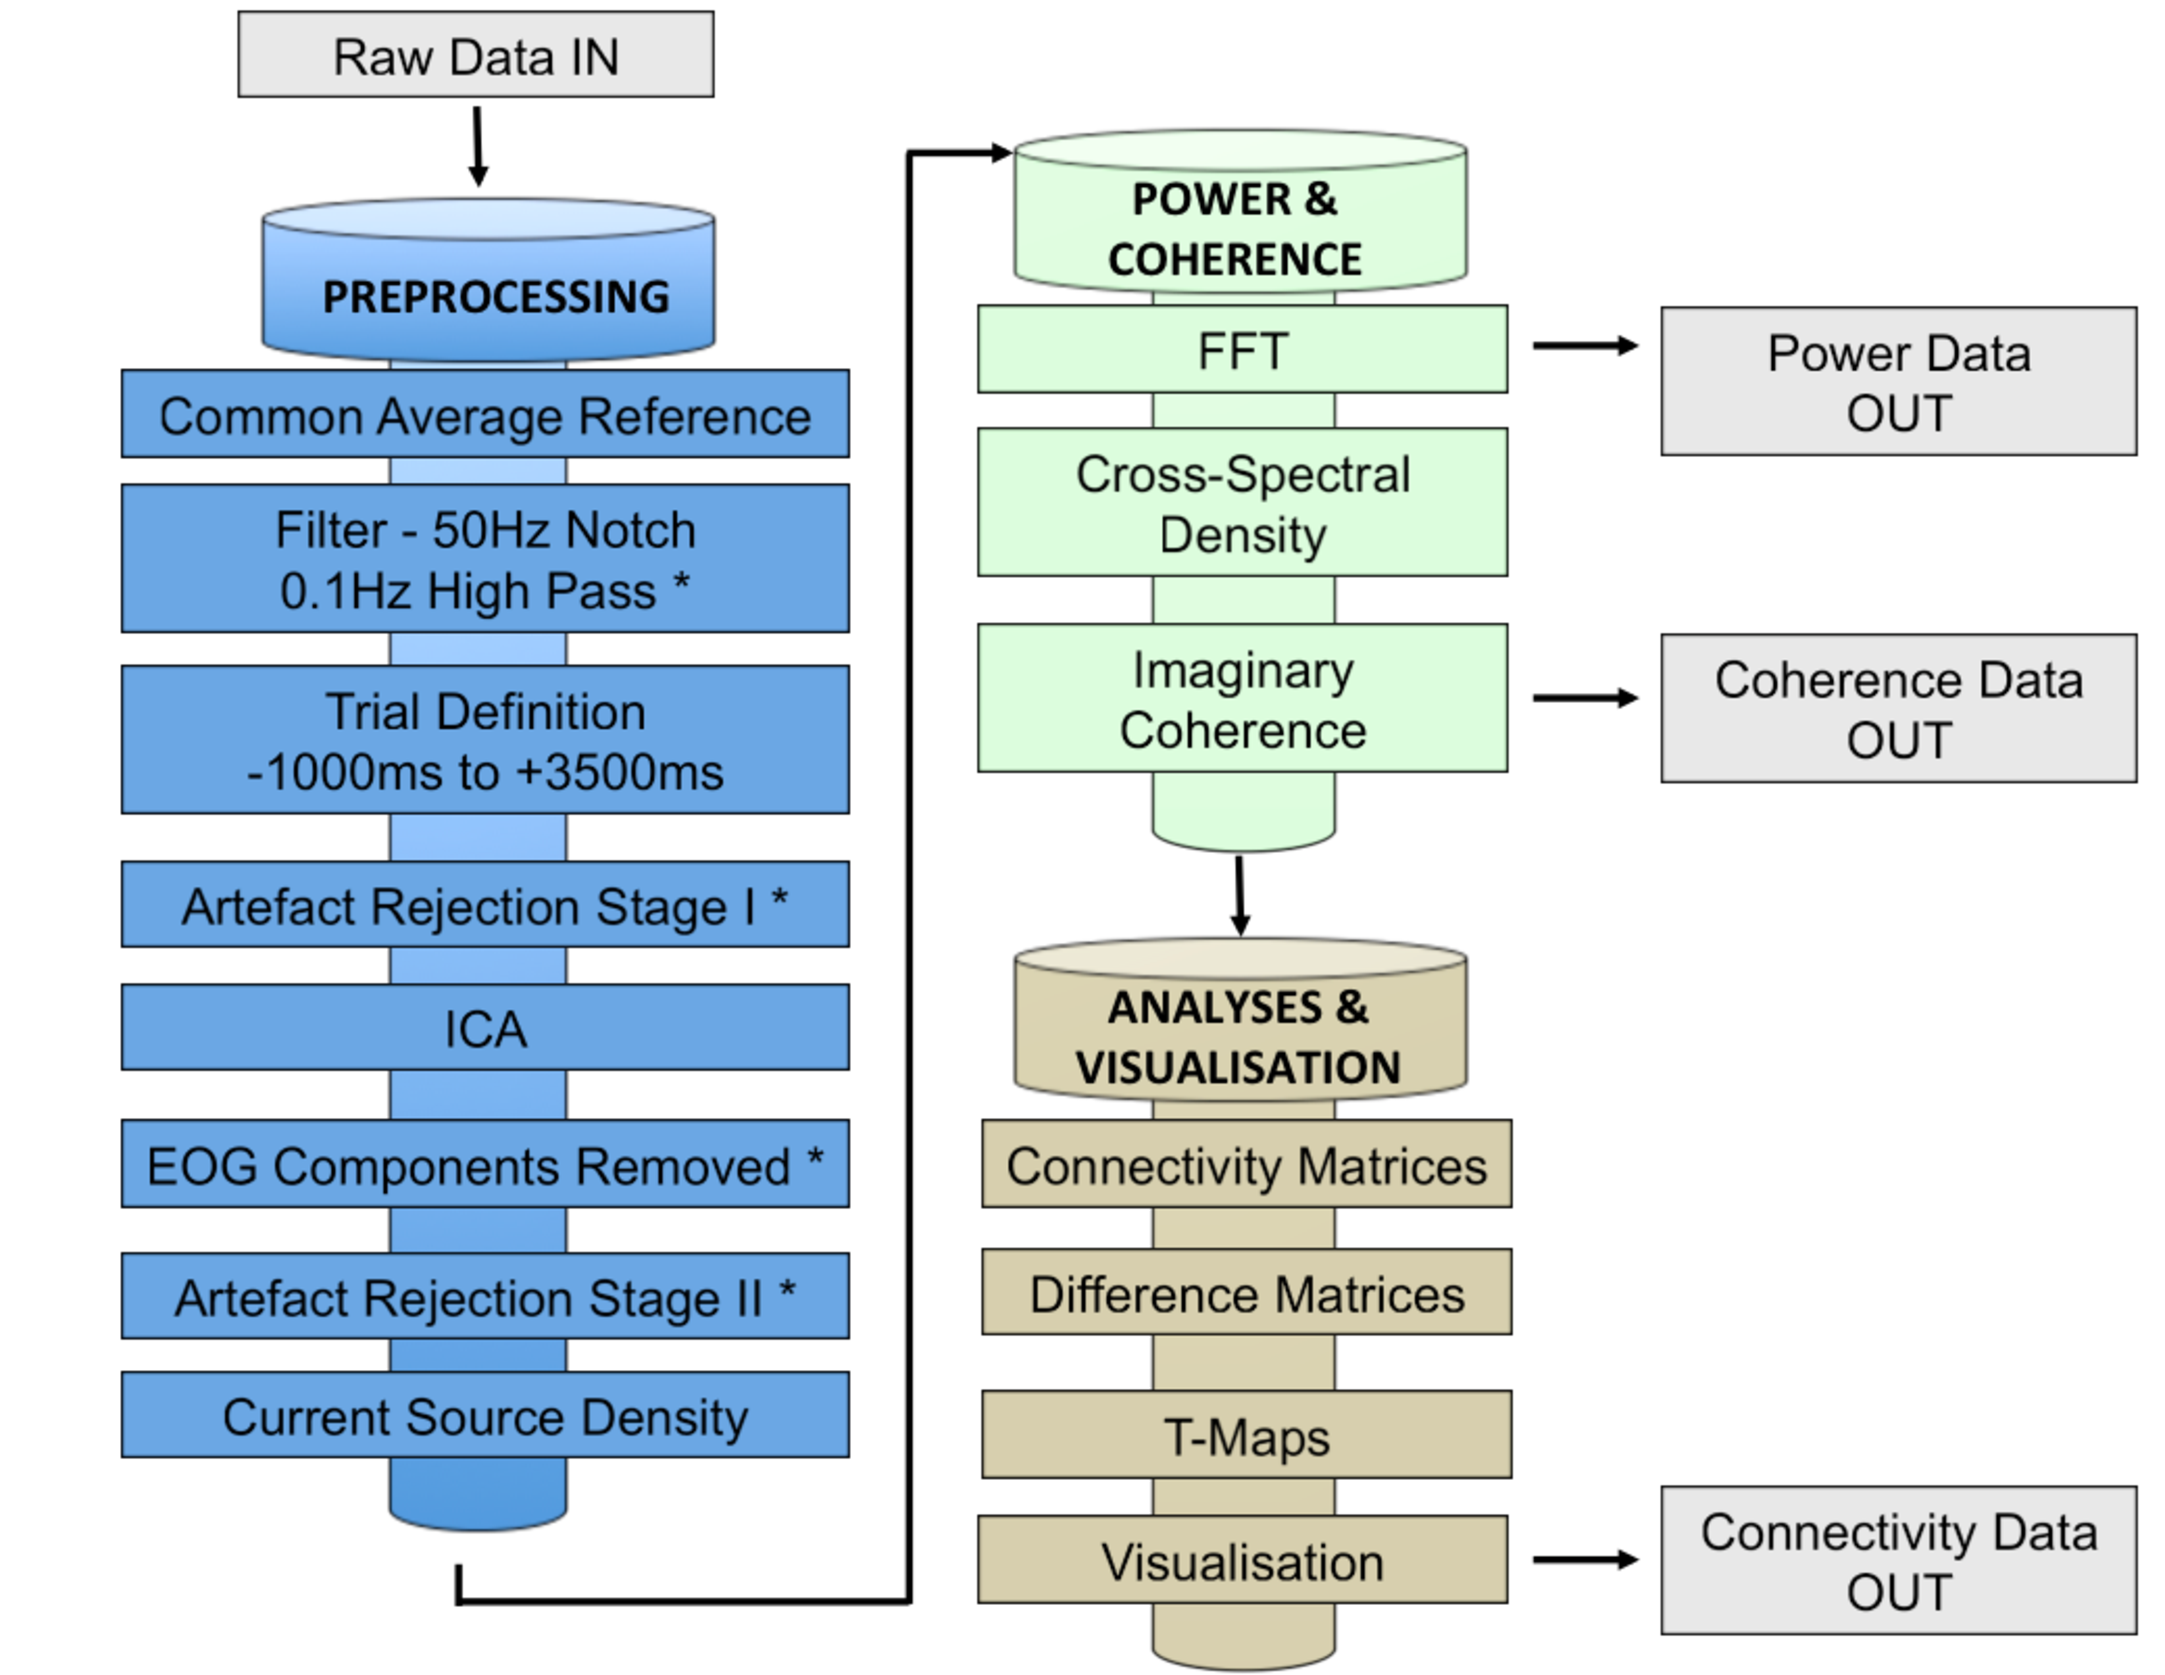
\includegraphics[width=90mm]{Figure2.pdf}
\caption{Processing pipeline for EEG analysis. EEG data were processed using an in-house developed, semi-automated pipeline utilising Fieldtrip (Blue), EEGLab (Green) and custom (Brown) routines. For details, refer to \emph{Methods}. * indicates processing stages requiring manual user visualistion.}
\label{Pipeline}
\end{figure}

\subsubsection{Power Analysis}

The power for each condition was calculated by transforming single-trial data into its time-frequency representation. To do so, we multiplied the power spectrum derived from a fast-Fourier transform (FFT), where frequencies were analysed across 80 logarithmically-spaced frequency bins, ranging from 2Hz to 50Hz, and time from 400ms pre-cue to 2,200ms post cue, by the power spectrum of Morlet wavelets:
\begin{equation}
e ^{i 2 \pi f}e^{\frac{-t^2}{(2\sigma^2)}}
\end{equation} where \emph{f} = the current frequency, \emph{t} = time and \emph{$\sigma$} = the width of each frequency band (\emph{n/(2$\pi$f)}), \emph{n} increases logairthmaicllay from 3 to 14 with respect to \emph{f}. An inverse FFT (iFFT) was performed on the output of the above steps. The output of the iFFT for each trial was normalised with a decibel transformation (\emph{normalised power = 10*log10[power/baseline]}) where baseline referred to the average activity from 200ms pre-cue to cue onset. 
\subsubsection{Coherence Analysis}
We used imaginary coherence as our measure of oscillatory synchronisation. Coherence refers to the normalised cross-spectral correlation between two time series, containing information relating to a) the absolute magnitude of the relationship and b) the complex component representing phase information. If we look solely at the complex component of coherence, we can explore phase coupling between two time series. As phase information is not sensitive to volume conduction effects \citep{Nolte2004}, we can use this information to explore neural interactions confidently at sensor space. Imaginary coherence was calculated by first computing the cross-spectral power density  between each pair of electrodes (\emph{$S_{ij}$(f)}) for each time point across the 80 frequency bins. We then divided the derived power by the the cross-spectral power for each pair of electrodes to compute imaginary coherence, using the following expression:

\begin{equation}
C_{ij}(f) = \frac{S_{ij}(f)}{(S_{ii}(f)S_{jj}(f))^{1/2}}
\end{equation}
and extracting the complex component.

We then defined a connectivity matrix for frequencies \emph{delta} ($\delta$; 2-4Hz), \emph{theta} ($\theta$; 4-7Hz), \emph{loweralpha} ($\alpha$1; 8-10Hz), \emph{upperalpha} ($\alpha$2; 10-13Hz) and \emph{beta} ($\beta$; 13-30Hz) by averaging the imaginary coherence output across the frequency band using a 100ms sliding window (window size = 200ms) from cue onset to 600ms post target. This resulted in 15 time ranges for each frequency (5) and each condition (4). As CSD correction can produce artefacts at edge electrodes, our final connectivity matrices included only those sites not on the cap peripherals (i.e. AF3, F1, F3, F5, AF4, AFz, Fz, F2, F4, F6, FC5, FC3, FC1, FC6, FC4, FC2, FCz, C1, C3, C5, Cz, C2, C4, C6, CP5, CP3, CP1, CP6, CP4, CP2, CPz, P1, P3, P5, P7, Pz, P2, P4, P6, P8, PO7, PO3, O1, Oz, POz, PO8, PO4 and O2). Finally, as our paradigm lacked a pure baseline condition, we converted each connectivity matrix into a difference matrix which compared connectivity in the current frequency*time*condition interaction to connectivity during the current frequency*time*repeat condition. 
\subsection{Statistical Analyses}
Statistics on coherence results were performed using map-wise \emph{t}-tests, with effects considered statistically significant using a false-discovery rate (FDR) correction of \emph{p \textless 0.005} \citep{FDR2001}, following the multiple comparison correction guidelines of \citet{Nolte2004}. Our FDR correction reflects a confidence that 99.5\% of values observed are true observations. We present findings from an early preparatory window (100-300ms) in the cue to target interval and a post target period between 200 to 400ms. As our hypotheses targeted theta and alpha synchronisation we only report results from these frequencies here.

\section{Results}
\subsection{Behavioural Results}
Behavioural data were analysed using a repeated- measures ANOVA (TRIAL TYPE (4) * TASK (3)) in SPSS. For RT there were significant main effects for TRIAL TYPE, \textit{F}$_{(3,84)}$ = 120.005, \textit{p} \textless 0.001 and TASK, \textit{F}$_{(2,56)}$ = 24.454, \textit{p} \textless 0.001 but their interaction did not reach significance. Repeat trials were performed faster than switch-to, \textit{F}$_{(1,28)}$ = 63.66, \textit{p} \textless 0.001, switch-away, \textit{F}$_{(1,28)}$ = 192.988, \textit{p} \textless 0.001 and noninformative trials, \textit{F}$_{(1,28)}$ = 423.066, \textit{p} \textless 0.001. Switch-to trials were faster than switch-away \textit{F}$_{(1,28)}$ = 152.19, \textit{p} \textless 0.001 and noninformative trials \textit{F}$_{(1,28)}$ = 11.37, \textit{p} = 0.002, and noninformative were performed faster than switch-away \textit{F}$_{(1,28)}$ = 32.435, \textit{p} \textless 0.001 (see Table 1).
Overall our participants were very accurate, with significant main effects only for TRIAL TYPE \textit{F}$_{(3,84)}$ = 7.362, \textit{p} \textless 0.001, driven primarily by repeat trial performance being more accurate than switch-to, switch-away and non-informative trials.
\begin{table}[t]
\centering
\begin{tabular}{l c c c}
 & RT(ms) & Accuracy\\
Trial & (SE) & (SE)\\
\hline
Repeat & 694.3&98.59\\
 & (21.65) &(.303) \\
SwitchTo & 817.35&96.5 \\
 & (32.3) & (.81)\\
SwitchAway & 927.26&96.64\\
 & (31.03) & (.885)\\
NonInformative & 858.73&96.84\\
 & (23.37) & (.589)\\
\hline
\end{tabular}
\caption{Means and standard errors for reaction time and accuracy across each of the four task switching trial types.}
\label{tab: template}
\end{table}

\subsection{Power Analyses}
In alpha but not theta frequency bands, switch specific power features were indentified during the cue to target interval. Figure 3 highlights the strongest of these effects, showing the increase in parietal power for switch-to and switch-away conditions in the upper alpha band (see Supplementary Materials for equivalent plots for theta and lower alpha bands).
Both switch-to and switch-away show marked increases in parietal power relative to the repeat baseline condition during the 400-600ms preparation interval that is largely absent for the noninformative condition. The strongest power is observed during this 400-600ms window but for switch-away trials in particular it is seen to wax and wane in the two adjacent time windows (200-400 and 600-800ms).
\begin{figure}
\centering
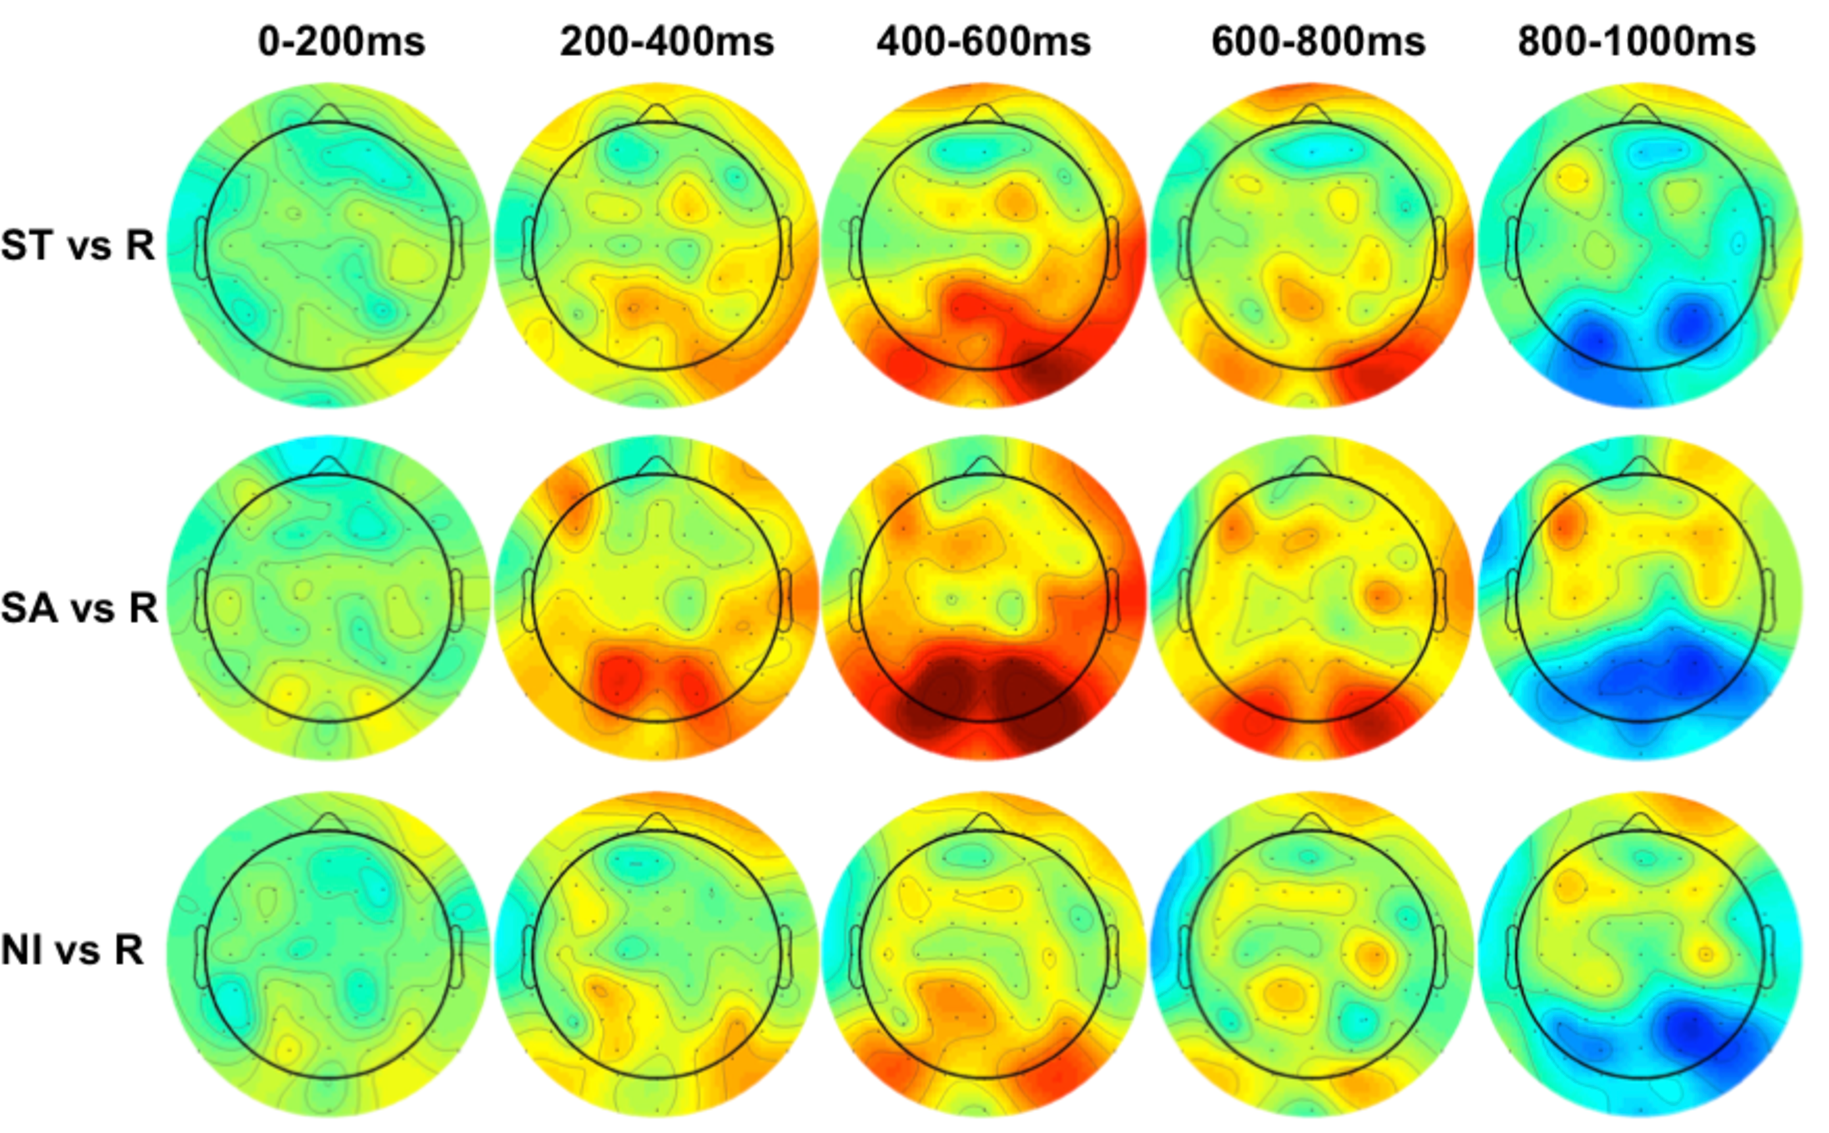
\includegraphics[width =0.5\textwidth]{UpperAlphaPower.pdf}
\caption{Power analysis in upper alpha (8-13Hz) during the cue to target preparatory interval. Both switch-to and switch-away conditions show large parietal increases in power during early preparation that is reduced/absent in noninformative trials. R, repeat; ST, switch-to; SA, switch-away; NI, noninformative.}
\label{Power}
\end{figure} 

\subsection{Imaginary Coherence Analyses}
Coherence differences for each trial type in theta, lower alpha and upper alpha bands are reported here relative to repeat conditions for an early preparatory window and a later post-target window. Significant \emph{t}-values corrected for multiple comparisons using FDR p\textless.005 are shown in Figures 4 and 5. Figure 4 shows extensive connectivity between parietal, frontocentral and frontal electrodes in switch-to and switch-away conditions during the early preparatory window (100-300ms post cue). A common set of switch-specific connections can be observed for switch-to and switch-away trials in both lower and upper alpha frequency bands. This frontoparietal network is absent for the alpha bands during early noninformative preparation, although there is some long range connectivity with a few parietal sites (Pz and P1) in the upper alpha band. Switch-related frontoparietal connectivity during this period is relatively sparse for theta band and again is concentrated on few frontal electrodes with high connectivity. Post-target (200-400ms after target onset) connectivity is shown in Figure 5, with extensive coherence between frontal, central and parietal sites in the theta band for switch-away and noninformative trials. Switch-to connectivity is virtually absent across all three frequencies. Finally, switch-away and noninformative frontoparietal connectivity is also missing for lower alpha and is minimal for upper alpha.
\begin{figure*}
\centering
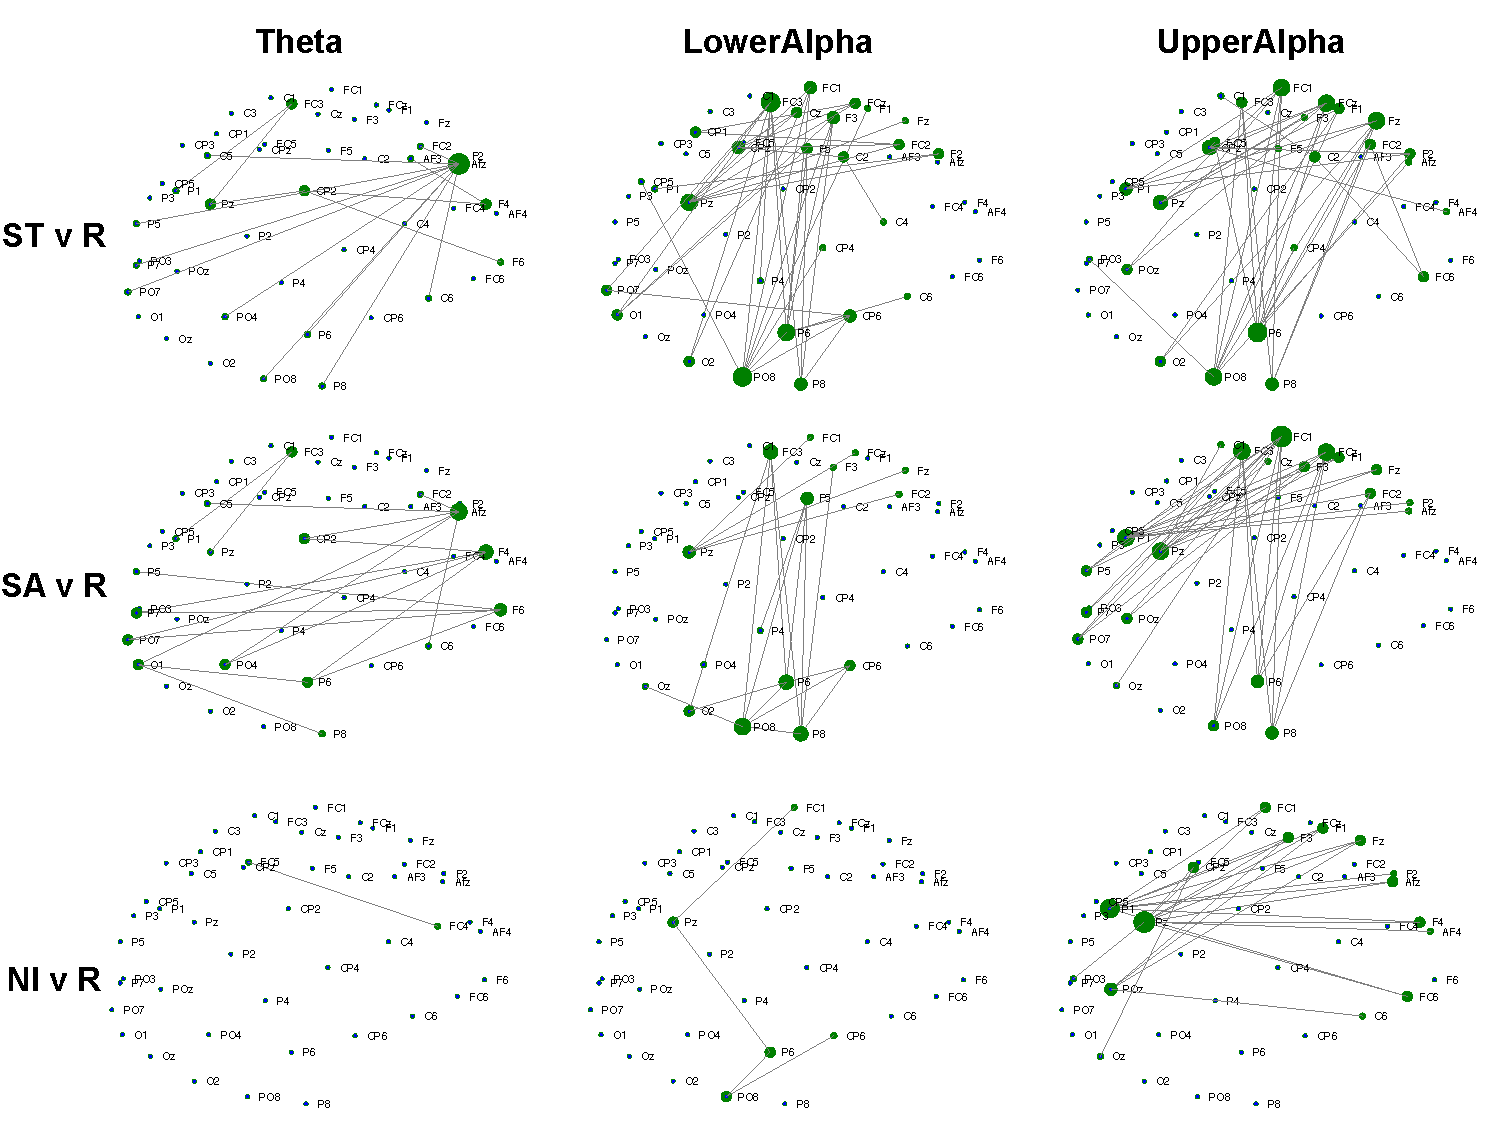
\includegraphics[width = 0.7\textwidth]{100to300_connplots.pdf}
\caption{Coherence during early preparation interval (100-300ms post cue). Electrode size is proportional to node degree (number of connections involving respective electrode). Lower alpha (8-10Hz) and upper alpha (10-13Hz) bands exhibit extensive frontoparietal connectivity for switching conditions. ST and SA share a common set of connections across alpha bands. Minimal connectivity present in theta band. R, repeat; ST, switch-to; SA, switch-away; NI, noninformative.}
\label{CueCoherence}
\end{figure*}

\begin{figure*}
\centering
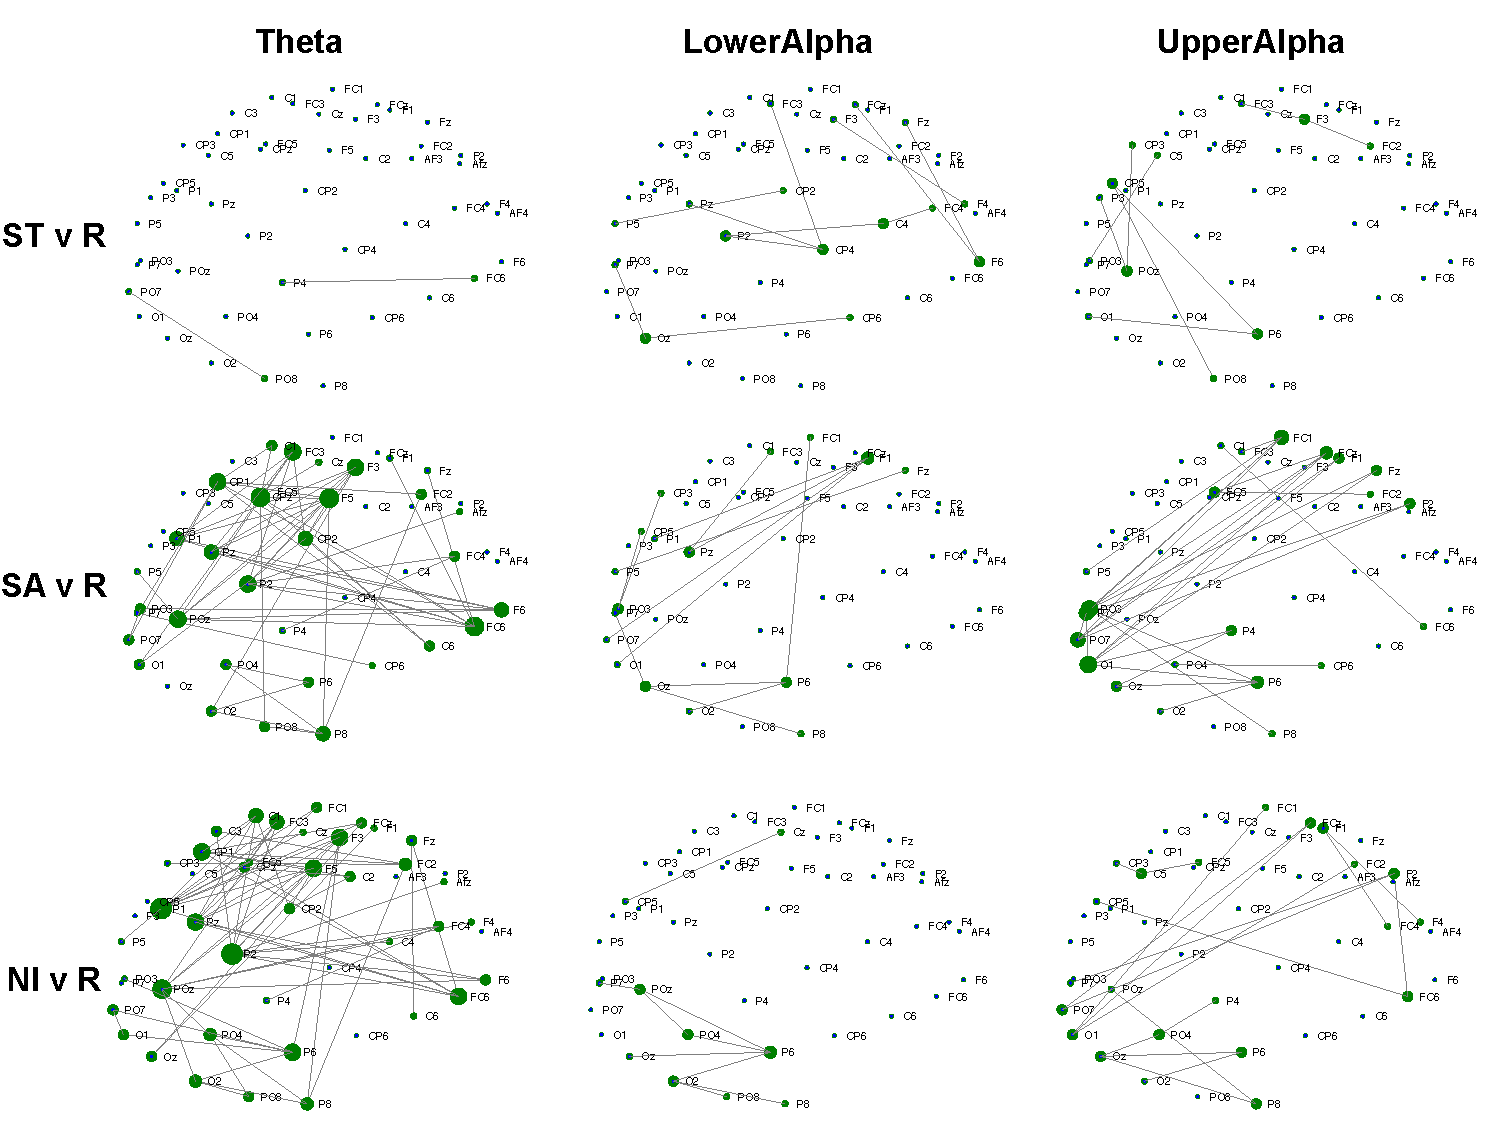
\includegraphics[width = 0.7\textwidth]{1200to1400_connplots.pdf}
\caption{Coherence after target onset (200-400ms post target). Extensive frontoparietal connectivity can be seen in switch-away and non-informative conditions for the theta band. Minimal connectivity present in alpha bands. R, repeat; ST, switch-to; SA, switch-away; NI, noninformative.}
\label{TargetCoherence}
\end{figure*}
\section{Discussion}
Although cognitive control can occur either proactively or reactively, studies examining the role of oscillatory synchronisation in control typically use paradigms that rely primarily on reactive control. These studies report frontoparietal synchronisation restricted to theta band communication (e.g. \citealt{Moore2006, Moore2012, SausengTSWT}) and so theta connectivity has been suggested to be a neural signature of goal-directed cognitive processes. Yet, the few studies that have explored whether this theta connectivity was present during proactive control suggested a role of alpha rather than theta activity during anticipatory control processes \citep{Mansfield2012,Serrien}. In the current study we aimed to determine whether the functional dissociation between proactive and reactive control had a similar dissociation in neural signatures. 

We found that indeed there was a dissociation between proactive and reactive control oscillatory synchronisation. During a cued trials task-switching paradigm preparing to switch tasks relied on extensive frontoparietal connectivity in lower and upper alpha bands but not in the theta band. In contrast, when there was insufficient information to completely anticipate the upcoming trial, extensive frontoparietal connectivity was observed in the theta but not alpha band after target onset. Together, proactive control, indexed by a need for an upcoming task-set switch, utilises frontoparietal alpha oscillatory synchronisation whereas reactive control, indexed by a need to resolve interference at target onset, utilises theta oscillatory synchronisation.

Previously, task switching was suggested to rely on frontoparietal theta oscillatory synchronisation, with theta synchronisaton reflecting control processes that permit working memory and long term memory storage interactions \citep{SausengTSWT}. We found a similarly structured theta band frontoparietal network as \citeauthor{SausengTSWT} for switch-away and noninformative conditions post-target but it was not present for switch-to trials. Our findings are therefore contrary to the above interpretation of theta, as the use of a cue allows task-set retreival processes to occur prior to target onset and so we should observe this theta connectivity during the cue to target preparation period. However, we only saw this switch-specific coupling in the alpha band and instead found frontoparietal connectivity in theta after target onset but not specifically to switch trials. 
\newpage
\section{References}
\bibliographystyle{elsarticle-harv}
\bibliography{Cooper_Library}



\end{document}